\chapter{Очереди работ}

\section{Реализация}

\begin{lstlisting}[caption={}]
#include <linux/init.h>
#include <linux/module.h>
#include <linux/kernel.h>
#include <linux/interrupt.h>
#include <linux/workqueue.h>

#define HANDLED_IRQ 1

MODULE_LICENSE("GPL");
MODULE_AUTHOR("Faris Nabiev");

static int  __init my_workqueue_init(void);
static void __exit my_workqueue_exit(void);

module_init(my_workqueue_init)
module_exit(my_workqueue_exit)

static int dev_id;
static int irq_call_cnt = 0;
// Очередь работ
static struct workqueue_struct *my_workqueue_struct;

// Функция обработки нижней половины
void my_workqueue_function(struct work_struct *work)
{
    printk(KERN_INFO "workqueue: counter %d\n", ++irq_call_cnt);
}

DECLARE_WORK(my_workqueue, my_workqueue_function);

// Обработчик прерывания
static irqreturn_t ihandler(int irq, void *dev_id)
{
    // Проверка, что произошло именно нужное прервыние
    if (irq == HANDLED_IRQ)
    {
        queue_work(my_workqueue_struct, &my_workqueue);
        printk(KERN_INFO "workqueue: in ihandler\n");

        return IRQ_HANDLED; // Прерывание обработано
    }
    else
        return IRQ_NONE; // Прерывание не обработано
}

static int __init my_workqueue_init(void)
{
    // Инициализация модуля
    if (request_irq(HANDLED_IRQ, ihandler,
                    IRQF_SHARED, "ihandler", &dev_id))
    {
        printk(KERN_ERR "workqueue: Error on handler registering\n");

        return -1;
    }

    // создание очереди работ
    my_workqueue_struct = create_workqueue("my_workqueue");

    if (!my_workqueue_struct)
    {
        free_irq(HANDLED_IRQ, &dev_id);
        printk(KERN_ERR "workqueue: Error on workqueue creation\n");

        return -ENOMEM;
    }

    printk(KERN_INFO "workqueue: workqueue created\n");
    printk(KERN_INFO "workqueue: Module loaded!\n");

    return 0;
}

// Выгрузка модуля
static void __exit my_workqueue_exit(void)
{
    // Удаление очереди работ
    flush_workqueue(my_workqueue_struct);
    destroy_workqueue(my_workqueue_struct);
    // Освобождение линии прерывания
    free_irq(HANDLED_IRQ, &dev_id);

    printk(KERN_INFO "workqueue: Module unloaded\n");
}
\end{lstlisting}

\section{Результаты работы}

\begin{figure}[H]
    \centering
    \caption{Сборка}
    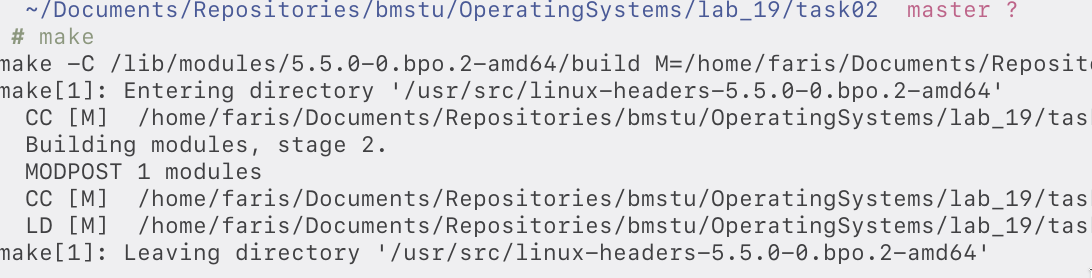
\includegraphics[scale=0.375]{images/scr2_1.png}
\end{figure}
\begin{figure}[H]
    \centering
    \caption{Загрузка модуля ядра, вывод буфера сообщений ядра, проверка списка загруженных модулей}
    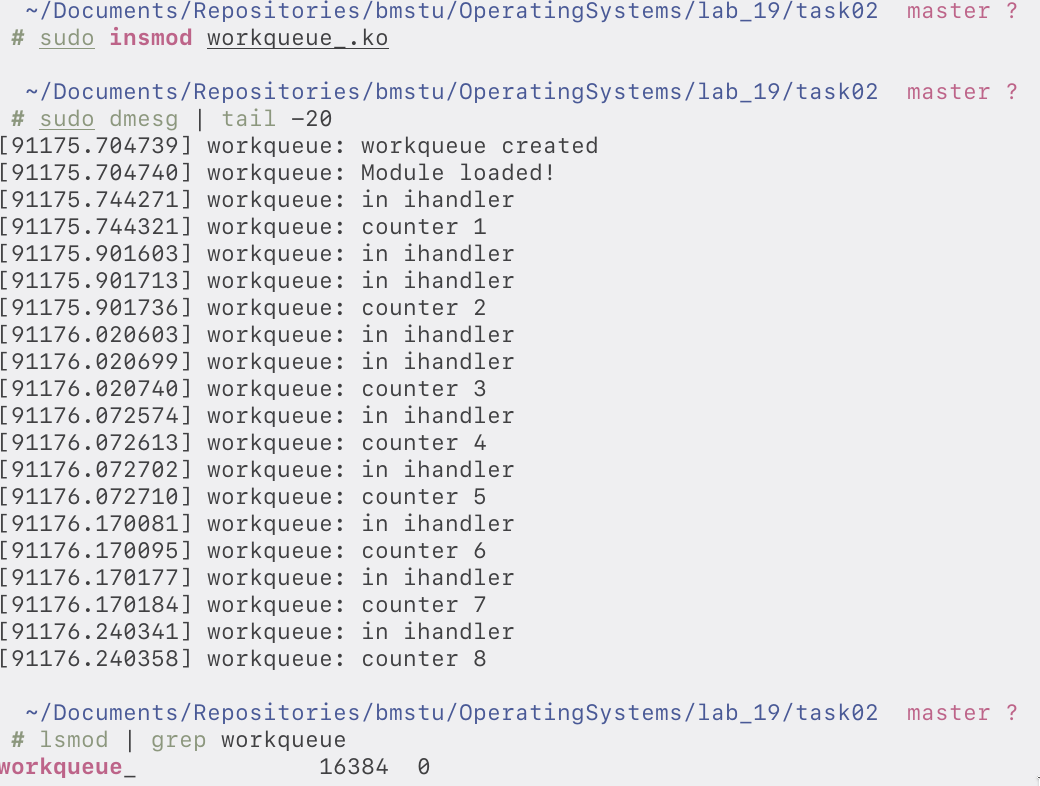
\includegraphics[scale=0.375]{images/scr2_2.png}
\end{figure}
\begin{figure}[H]
    \centering
    \caption{Просмотр содержимого /proc/interrupts}
    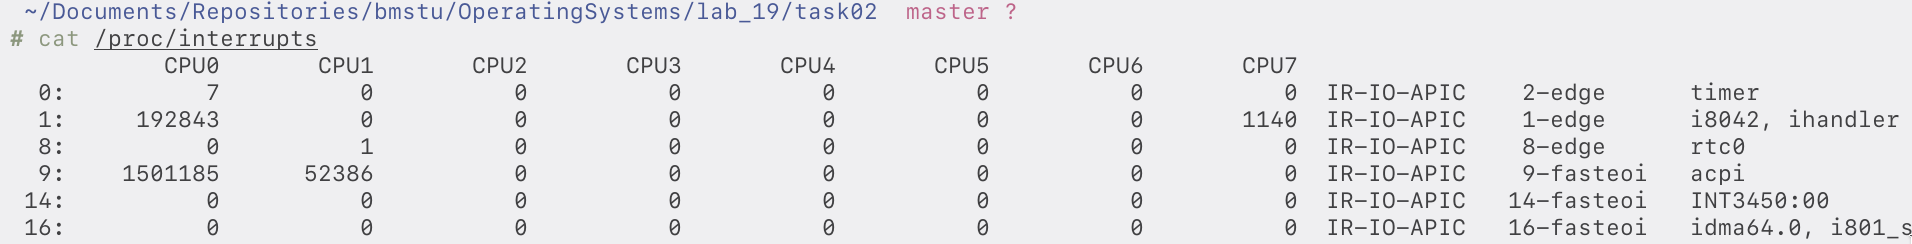
\includegraphics[scale=0.235]{images/scr2_3.png}
\end{figure}
\begin{figure}[H]
    \centering
    \caption{Выгрузка модуля ядра, вывод буфера сообщений ядра}
    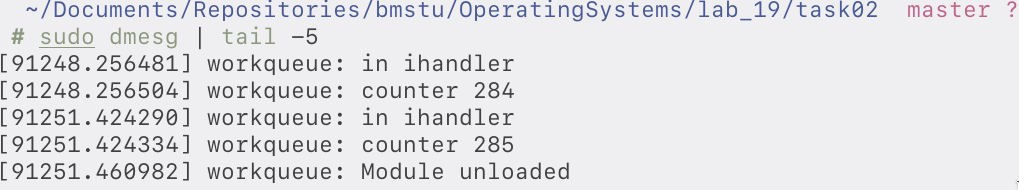
\includegraphics[scale=0.375]{images/scr2_4.png}
\end{figure}
